 \documentclass{beamer}
%\documentclass[handout]{beamer}
\usetheme{metropolis}

%\setbeameroption{show notes}

\usepackage{pgfpages}
\setbeameroption{show notes on second screen}

% Packages
\usepackage[utf8]{inputenc}

\usepackage{animate}

\usepackage{appendixnumberbeamer}
\usepackage{xcolor}
\usepackage{multirow}
% Maths
\usepackage{amsthm}
\usepackage{tikz}
\usetikzlibrary{cd}

% References
\usepackage{biblatex}
\addbibresource{./references.bib}

% Package Settings
% AMSTHM
\theoremstyle{plain}
\newtheorem{thm}{Theorem}[section]
\newtheorem{mylemma}[thm]{Lemma}
\newtheorem{cor}[thm]{Corollary}
\newtheorem{rem}[thm]{Remark}
\newtheorem{alg}[thm]{Algorithm}

\theoremstyle{definition}
\newtheorem{defn}[thm]{Definition}

\newcommand{\todo}[1]{{\color{red}*** #1 ***}}

\renewcommand{\phi}{\varphi}

% BEAMER
% Hack for only and tabular
\newcommand{\tabularonly}{AS}
% Hack for tilde and hat
\newcommand{\mytilde}[1]    {\ensuremath{\tilde{#1}}}
\newcommand{\myhat}[1]    {\ensuremath{\widehat{#1}}}
% Hack to display \Gamma with a little bit of space to the left
% Otherwise \ind _ \Gamma ^ H looks really weird
\let\oldGamma\Gamma
\renewcommand{\Gamma}{{\hspace{0.5pt} \oldGamma}}
% Hack to reference the notation-definition in "lift a.s. normaliser"
\newcommand{\refdef}    {{(6.1)}}

% Symbols
% Write function definitions like
% f \from A \to B
\newcommand{\from}	{\ensuremath{\colon}}
\renewcommand{\to}	{\ensuremath{\rightarrow}}
\newcommand{\into}	{\ensuremath{\hookrightarrow}}
\newcommand{\onto}	{\ensuremath{\twoheadrightarrow}}
\newcommand{\iso}	{\ensuremath{\xrightarrow{\,\raisebox{-1pt}{\ensuremath{\scriptstyle{\sim}}}\,}}}
\newcommand{\N}	{\ensuremath{\mathbb N}}
\newcommand{\Z}	{\ensuremath{\mathbb Z}}
\newcommand{\Q}	{\ensuremath{\mathbb Q}}
\newcommand{\Sn}{{\ensuremath{\mathrm{S}_n}}}
\newcommand{\uln} {{\ensuremath{\underline n}}}

%%% Categories
\newcommand{\permgrp}   {\ensuremath{\mathbf{PermGrp}}}

%%% Unary Operators
% Functions
\DeclareMathOperator{\dom}{dom}
\DeclareMathOperator{\id}{id}
\DeclareMathOperator{\im}{Im}
% Groups
\DeclareMathOperator{\sym}{Sym}
\DeclareMathOperator{\Sym}{Sym}
\DeclareMathOperator{\alternating}{Alt}
\DeclareMathOperator{\Alt}{Alt}
\DeclareMathOperator{\soc}{soc}
\DeclareMathOperator{\aut}{Aut}
\DeclareMathOperator{\Aut}{Aut}
\DeclareMathOperator{\out}{Out}
\DeclareMathOperator{\Out}{Out}
\DeclareMathOperator{\ind}{Ind}
\DeclareMathOperator{\res}{Res}
\DeclareMathOperator{\stab}{Stab}
\newcommand{\hatOperator}   {\ensuremath{\, \myhat \cdot\,}}
\def\Norm#1#2{\mathrm{N}_{#1}(#2)}

%%% Binary Operators %%%
\newcommand{\union}{\mathbin{\cup}}
\newcommand{\bigunion}{\mathbin{\bigcup}}
\newcommand{\disjointunion}{\mathbin{\uplus}}
\newcommand{\intersection}{\mathbin{\cap}}
\newcommand{\bigintersection}{\mathbin{\bigcap}}
\newcommand{\norm}{\mathbin{\lhd}}
\newcommand{\characteristic}{\mathbin{\text{char}}}


% New commands
\newcommand{\abs}[1]	{%
	\ensuremath{
		\left| #1 \right|
	}%
}
\newcommand{\gen}[1]	{
	\ensuremath{
		\left\langle \, #1 \, \right\rangle
	}
}
\newcommand{\set}[1]	{
	\ensuremath{
		\left\{ #1 \right\}
	}
}
\newcommand{\sset}[2] {
	\ensuremath{
		\left\{ \left.\,
			#1
		~\right|~
			#2
		\,\right\}
	}
}


\title{Normalizers of simple diagonal groups in polynomial time}
\subtitle{Groups and Combinatorics Seminar}
\date{July 30th, 2021}
\author{Sergio Siccha}
\institute{TU Kaiserslautern}

\begin{document}

\maketitle
\note{
RECORDING
\\
RECORDING
\\
RECORDING
\\
}

\section{Introduction}

\begin{frame}{Representation}

Groups are given by generating sets of permutations.

Compute a group: compute a generating set.

Permutation groups are given on points $\set{1, \ldots, n}$.

\end{frame}

\begin{frame}{Normalizers}
Let $G, M \leq K$ be groups.
The \emph{normalizer of $G$ in $M$} is
the group
\[
N_M(G) = \set{ m \in M ~|~ G ^ m = G }.
\]

\pause
\emph{Normalizer problem}: Given $G, M \leq S_n$, compute $N_M(G)$.

\pause
In practice partition backtrack.

Best known theoretical algorithm by D. Wiebking for
$N_{S_n}(G)$ in
time $2 ^ {O(n)}$.
\end{frame}

\note{
Luks and Miyazaki 2011
}


\begin{frame}{Motivation}
Normalizers remain hard in practice and in theory.

Permutation morphisms are very nice tools.
\end{frame}

\note{Babai 2016}

\begin{frame}{Primitive Groups}
A transitive group $G \leq \Sym \Omega$ is
\emph{imprimitive}, if there exists a non-trivial $G$-invariant partition of
$\Omega$,
otherwise it is \emph{primitive}.

\begin{columns}
\begin{column}{0.5\textwidth}
$D_8 := \gen{ (1,2,3,4),\, (1,4)(2,3) }$
\\[1em]

$\set{ \set{1,3}, \set{2,4} }$ is $D_8$-invariant.
\end{column}
\begin{column}{0.3\textwidth}
{
\only<1->{
\begin{figure}[h]
\centering
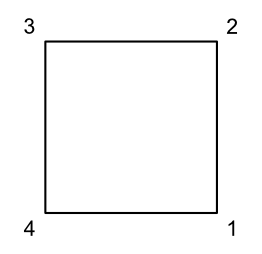
\includegraphics[width=0.9\textwidth]{./pictures/square.png}
\caption{A square}
\end{figure}
}
}
\end{column}
\end{columns}
\end{frame}

\begin{frame}%{Resultat}
\begin{block}{Theorem (S. 2020)}
Let $G = \gen X \leq \Sym \Omega$ be a primitive group
with non-regular socle.
We can compute (a generating set of) $N_{\Sym \Omega}(G)$
in time $O(\abs X \abs \Omega ^ c)$.
\end{block}
\vspace{1em}
\pause
Note: For $M \leq \sym \Omega$ we have
$N_{M}(G) = M \cap N_{\sym \Omega}(G)$.

\vspace{1em}
\pause
For these groups, computing the normalizer is as hard as computing
intersections.
\end{frame}

%\begin{frame}{Implementation}
%A partial implementation is available at the github repository
%\begin{center}
%\href{https://github.com/ssiccha/NormalizersOfPrimitiveGroups}
%{\textcolor{blue}{ssiccha/NormalizersOfPrimitiveGroups}}
%\end{center}
%\vspace{1\baselineskip}
%
%$N_{\Sym \Omega}(G)$ for $G$ primitive with $\abs \Omega = 5 ^ 7 = 78125$ in
%$\approx 67 s$.
%\end{frame}


\section{Strategy}
\begin{frame}{Standing on the shoulders of giants}
Ingredients:
\begin{itemize}
\item O'Nan-Scott Theorem
\item Classification of finite simple groups (CFSG)
\end{itemize}

\pause
Problem:
\begin{itemize}
\item Use O'Nan-Scott algorithmically
\end{itemize}

\end{frame}

\note{For other types: reconstruct the component-wise action}

\begin{frame}
Let $\Delta := \set{1, \ldots, 5}$ and
$X \leq S_{125}$ be permutation isomorphic to
$(A_5) ^ 3 \leq \sym(\Delta ^ 3)$ in component-wise action.

If the permutation isomorphism is ``send a tuple to its $5$-adic expansion
(with offset)'',
\pause
then we have
\begin{align*}
    &(1, 2, 3, 4, 5) (6, 7, 8, 9, 10) \ldots \in X
    \\
    &(1, 6, 11, 16, 21) (2, 7, 12, 17, 22) \ldots \in X
\end{align*}

\pause
If the permutation isomorphism is not ``nice'' we might have
\begin{align*}
    &(1, 123, 79, 11, 55) (2, 3, 23, 63, 78) \ldots \in X.
\end{align*}
\end{frame}

\note{``not nice'' could have an arbitrary conjugate of the ``nice'' group}

\begin{frame}{Classification of primitive groups}
Let $G$ be a group. The \emph{socle} of $G$, denoted $\soc G$,
is the group generated by all minimal normal subgroups of $G$.

The socle of a primitive group is a direct power of a simple group.
\pause
\begin{block}{O'Nan-Scott Theorem}
    Let $G \leq S_n$ be primitive.
    Then $\soc G \leq G \leq N_{S_n}(\soc G)$
    and we know all possible permutational isomorphism types of
    \vspace{-0.5em}
    \begin{itemize}
        \item
        $\soc G$ and
        \item
        $N_{S_n}(\soc G)$.
    \end{itemize}
\end{block}
\end{frame}

\note{
For type AS this doesn't yield any information.
}

\begin{frame}{Main steps}
Goal:
\\
Let $G \leq S_n$ be primitive with non-regular socle.
Compute $N_{S_n}(G)$.

Algorithm:
\begin{enumerate}
\item Find a ``nice'' permutation isomorphism for $\soc G$
\\
(weak canonical form).

\item $M := N_{S_n}(\soc G)$.
Then we have $N_{S_n}(G) = N_M(G)$.

\item
$
    \rho : M \to S_k
$
with $k \leq c \cdot \log n$.
Use Wiebking's $2 ^ {O(n)}$ algorithm.
\end{enumerate}
\vspace{1em}

\pause
Today: focus on step 2 for primitive groups of type SD.
\end{frame}

\note{Step 1: reconstruct component-wise action of the socle ( or a suitable
big normal subgroup )
\\
Step 3: Transform product action wreath product into a primitive wreath
product: $m ^ d$ points to $m \cdot d$ points.
Thus $d \sim \log_m n$.
Then factor out the socle such that the outer automorphisms contribute
only a factor of $\log m$.
In total: $\log m \cdot \log_m n = \log n$.
\\
Step 2 today: only present tool for correctness.}

\section{Permutation morphisms}
\begin{frame}{Language}
``[...] many properties of mathematical systems can be unified and simplified
by a presentation with diagrams of arrows.''

\hfill --
Saunders Mac Lane
% Categories for the working mathematician, Introduction
\hspace{2em}

\vspace{2em}
\pause
``Language serves not only to express thoughts, but to make possible thoughts
which could not exist without it.''

\hfill --
Bertrand Russell
% Human Knowledge: Its Scope and Limits, p 74 as found in google books
\hspace{2em}
\end{frame}
\note{always superior? No, I tried to formulate the concept of "a group leaves
a cartesian decomposition invariant" with diagrams of arrows.
That did not work out.}

\begin{frame}{Three groups}
Let $T \leq \sym \Delta$ be a regular non-abelian finite simple group.

$T ^ \ell$ acts right-regularly on itself.

Let $G \leq \sym(\Delta ^ \ell)$ be a primitive group after
``step 1'' and $H = \soc G$.

%Let $C := C_{\sym \Delta}(T)$,
%$\diag_{\ell - 1}(C) = \sset{(c, \ldots, c) \in C ^ {\ell - 1}}{ c \in C }$,
%and
%$H := \gen{ T ^ {\ell - 1}, \diag_{\ell - 1}(C) } \leq
%\sym(\Delta ^ {\ell - 1})$.

Let $\mathcal D$ be the group induced by the \emph{standard diagonal action} of $T ^ \ell$.

\pause
\[
\begin{tikzcd}[column sep=small, ampersand replacement=\&]
    \&
    T ^ \ell
    \&
    \\
    H
    \&
    \&
    \mathcal D
\end{tikzcd}
\]
\end{frame}

\note{If not algorithmic, then there are only $T ^ \ell$ and $\mathcal D$.
We can identify these, no problem.
Three groups though is too much for identification IMO.
So we need to translate between these three worlds.}

\begin{frame}{Permutation isomorphism (1)}
Let $G \leq \sym \Omega$ and $H \leq \sym \Delta$.
We call $(f, \varphi)$ with
isomorphisms
$f \from \Omega \iso \Delta$
and
$\varphi \from G \iso H$
a \emph{permutation isomorphism}
from $G$ to $H$
if
$\forall g \in G, ~ \forall \omega \in \Omega :$
\[
    f(\omega ^ g) = f(\omega) ^ {\varphi(g)}.
\]
\end{frame}

\begin{frame}{Permutation isomorphism (2)}
Let
$f \times \varphi \from (\omega, g) \mapsto (f(\omega), \phi(g))$.

\pause
Let $\rho \from \Omega \times G \to \Omega$ and
$\tau \from \Delta \times H \to \Delta$ be \textbf{natural} actions,
and
$f, \phi$ be as before.
\pause
Then $(f, \phi)$ is a \emph{permutation isomorphism}
if and only if:
\vspace{1em}
\[
\begin{tikzcd}[ampersand replacement=\&]
    \Omega \times G
        \ar[r, "\rho"]
        \ar[d, "f \times \varphi"]
    \&
    \Omega
        \ar[d, "f"]
    %
    \\
    %
    \Delta \times H
        \ar[r, "\tau"]
    \&
    \Delta
\end{tikzcd}
\raisebox{-2em}{.}
\]
\end{frame}

\begin{frame}{Permutation morphism}
Let $\rho \from \Omega \times G \to \Omega$ and
$\tau \from \Delta \times H \to \Delta$ be \textbf{natural} actions.
We call $F = (f, \phi)$ with
$f \from \Omega \to \Delta,~ \phi \from G \to H$
a \emph{permutation morphism} from $G$ to $H$
if:
\vspace{1em}
\[
\begin{tikzcd}[ampersand replacement=\&]
    \Omega \times G
        \ar[r, "\rho"]
        \ar[d, "f \times \varphi"]
    \&
    \Omega
        \ar[d, "f"]
    %
    \\
    %
    \Delta \times H
        \ar[r, "\tau"]
    \&
    \Delta
\end{tikzcd}
\raisebox{-2em}{.}
\]
\end{frame}

\begin{frame}{Action morphism}
Let $\rho \from \Omega \times G \to \Omega$ and
$\tau \from \Delta \times H \to \Delta$ be actions.
We call $F = (f, \phi)$ with
$f \from \Omega \to \Delta,~ \phi \from G \to H$
an \emph{action morphism}
if:
\vspace{1em}
\[
\begin{tikzcd}[ampersand replacement=\&]
    \Omega \times G
        \ar[r, "\rho"]
        \ar[d, "f \times \varphi"]
    \&
    \Omega
        \ar[d, "f"]
    %
    \\
    %
    \Delta \times H
        \ar[r, "\tau"]
    \&
    \Delta
\end{tikzcd}
\raisebox{-2em}{.}
\]

\end{frame}

\begin{frame}{Composition}
Componentwise:
\[
\begin{tikzcd}[ampersand replacement=\&]
    \Omega \times G
        \ar[r, "\rho"]
        \ar[d, "f \times \varphi"]
    \&
    \Omega
        \ar[d, "f"]
    %
    \\
    %
    \Delta \times H
        \ar[r, "\tau"]
        \ar[d, "g \times \psi"]
    \&
    \Delta
        \ar[d, "g"]
    %
    \\
    %
    \Gamma \times K
        \ar[r, "\nu"]
    \&
    \Gamma
\end{tikzcd}
\raisebox{-3em}{.}
\]
\end{frame}

\begin{frame}{Categories}
\begin{block}{Proposition (S.)}
\begin{itemize}
\item Right-actions together with action morphisms form a category.
\item
Permutation groups together with permutation morphisms form a category.
That category admits finite products.
\end{itemize}
\end{block}
\end{frame}

\note{categories also are lots of fun,
admits = ``existence'', finite products used in PA case}

\begin{frame}{Permutation morphisms}
\begin{block}{Lemma (S.)}
Let $G \leq \sym \Omega$ and $f : \Omega \onto \Delta$.
There exist a (unique) group $H \leq \Sym \Delta$ and a (unique)
group epim. $\phi : G \to H$ such that
$(f, \phi)$ is a permutation epimorphism
if and only if:
\[
    \Sigma := \set{ f ^ {-1}(\set{\delta}) ~|~ \delta \in \Delta }
\]
is $G$-invariant.
\end{block}

%We call such an $f$ \emph{compatible} with $G$.

\pause
If $G$ transitive: $H = G ^ \Sigma$, $\phi : g \mapsto g ^ \Sigma$.
\end{frame}

\note{$\onto$ means surjective}

%\begin{frame}{Primitive groups and permutation morphisms}
%Note:
%a group $G$ is simple iff. all group homomorphisms
%$\phi : G \to H$ are trivial or injective.
%
%\begin{block}{Lemma (S.)}
%A permutation group $G$ is primitive iff. all permutation morphisms
%$F : G \to H$ are trivial or injective. we have $\ker \phi = \set{1_G}$ or $\ker \phi = G$.
%\end{block}
%a group admits only trivial group homomorphisms and group isomorphisms
%\end{frame}

\begin{frame}{Push-forward action}
\begin{block}{Definition}
Let $\rho : \Omega \times G \to \Omega$ be an action.
Let $f : \Omega \onto \Delta$ be surjective such that there exists
an action $\tau : \Delta \times G \to \Delta$ with
$(f, \id_G)$ being a morphism from $\rho$ to $\tau$.

We call $\tau$ the \emph{push-forward of $\rho$ by $f$}.
\end{block}
\end{frame}

%\begin{frame}{Permutation morphisms and products}
%\todo{push-forward example?}
%
%\begin{block}{Example}
%$\Omega := \set{1, \ldots, 4}$ und
%$V := \langle a := (1,2)(3,4),~$%
%$b := (1,3)(2,4) \rangle$.
%
%\begin{figure}[H]
%\centering
%\begin{tikzpicture}
%    % nodes
%    \foreach \x in {1, ..., 2}
%        \foreach \y in {1, ..., 2}
%            \draw [fill] (\x, \y) circle [radius=0.050];
%    \node [above left] at (1, 2) {{$1$}};
%    \node [above left] at (2, 2) {{$2$}};
%    \node [above left] at (1, 1) {{$3$}};
%    \node [above left] at (2, 1) {{$4$}};
%\end{tikzpicture}
%\end{figure}
%
%\only<1>{\vspace{9.25em}}
%\only<2>{
%\begin{align*}
%p_1 &: \Omega \to \set{1,3},~~
%1,2 \mapsto 1, ~~ 3,4 \mapsto 3,
%\\
%\pi_1 &: G \to \gen{(1,3)},~~
%\id_\Omega, a \mapsto \id_{\set{1,3}},
%~~b, ab \mapsto (1,3).
%\end{align*}
%
%Analoguously $P_2$.
%Then $P_1 \times P_2 : V \iso \gen{(1,3)} \times \gen{(1,2)}$
%}
%\only<3>{
%For
%$p_1' : \omega \mapsto \omega ^ {\gen{a}}$
%we have
%\begin{align*}
%1 ^ {\gen a} = 2 ^ {\gen a} = \set{ 1,2 }
%\\
%3 ^ {\gen a} = 4 ^ {\gen a} = \set{ 3,4 }
%\end{align*}
%\vspace{0.75em}
%}
%\end{block}
%\end{frame}

%\begin{frame}{Permutation morphisms and products}
%$\Delta = \set{1, \ldots, 5}$, $\Omega = \Delta ^ 2$,
%$H = (A_5) ^ 2 \leq \Sym(\Delta ^ 2)$,
%$N_1 := \mathbf 1 \times A_5 \unlhd H$.
%\end{frame}

%\begin{frame}{AS Type}
%Let $G \leq \sym \Omega$ be primitive.
%We say $G$ is of \emph{type AS}, if
%there exist a non-regular non-abelian simple group
%$T \leq \sym \Omega$ with $\soc G = T$.
%
%Use constructive recognition to compute $N_{\sym \Delta}(T)$.
%\end{frame}

%\begin{frame}{PA Type}
%Let $G \leq \sym \Omega$ be primitive.
%We say $G$ is of \emph{type PA}, if
%there exist a non-abelian simple group
%$T \leq \sym \Delta$
%and a permutation iso.
%$(f : \Omega \to \Delta ^ \ell,~ \phi : G \to H)$
%with
%\[
%\phi (\soc G) = T ^ \ell \leq \sym(\Delta ^ \ell).
%\]
%
%\pause
%\begin{block}{Corollary}
%$G \leq \sym(\Delta ^ \ell)$ primitive s.t.
%$\soc G = T ^ \ell$.
%Let $M := N_{\sym (\Delta ^ \ell)}(T ^ \ell)$.
%Then
%\[
%    M = N_{\sym \Delta}(T) \wr S_\ell
%\]
%and thus $M / (\soc G) \into \Out(T) \wr S_\ell$.
%\end{block}
%\end{frame}
%
%\begin{frame}{PA Type}
%\begin{block}{Step 1}
%Let $G \leq \sym(\Delta ^ \ell)$ primitive with
%$\soc G = T ^ \ell$.
%Then $M = N_{\Sym \Delta}(T) \wr S_\ell$ can be computed in polynomial
%time.
%\end{block}
%\vspace{1em}
%
%\pause
%\begin{block}{Step 2}
%\vspace{-1em}
%\[
%    M \to \Sym( \Delta \times \set{1, \ldots, \ell} ).
%\]
%\pause
%Theoretical version: Let $d := \abs \Delta$.
%Then $\abs{\Out T} \leq 3 \log d$ by
%\cite{guralnick-maroti-pyber:normalizers-primitive-groups}
%and $\ell = \log_d(n)$.
%\[
%    M \to \Out T \wr S_\ell \to S_{(3 \log n)}.
%\]
%\end{block}
%\end{frame}
%
%\begin{frame}
%How to find $T ^ \ell$ if $G \leq \Sym \Omega$ is arbitrary?
%Find $\ell$ \emph{projections} $\pi_i : \soc G \onto T$
%such that
%\[
%\prod \pi_i : \soc G \iso T ^ \ell
%\]
%yields a permutation isomorphism.
%\end{frame}

\section{Primitive groups of type SD}

\note{now keep notation for rest of talk}

\begin{frame}{Standard diagonal action (1)}
Let $T \leq \sym \Delta$ always be regular finite
non-abelian simple.

For $x \in T ^ \ell$ let
\[
    [x_1, \ldots, x_\ell]
    :=
    \sset{(t ^ {-1} x_1, \ldots, t ^ {-1} x_\ell)} {t \in T}
    \subseteq T ^ \ell.
\]

Call
\[
    \Sigma
    :=
    \sset{ [x_1, \ldots, x_\ell] }{ x \in T ^ \ell }
\]
and
\[
    d \from T ^ \ell \to \Sigma,
    (x_1, \ldots, x_\ell)
    \mapsto
    [x_1, \ldots, x_\ell].
\]

\pause
Call the push-forward by $d$
of the right-regular action of $T ^ \ell$
the \emph{(standard) diagonal action of $T ^ \ell$ (on $\Sigma$)}.
Let $\mathcal D$ be the group induced by $T ^ \ell$ on $\Sigma$.
\end{frame}

\note{$\mathcal D$ plays the role of the socle, take representative by fixing
last component to $1_T$.}

\begin{frame}{Standard diagonal action (2)}
\[
    [x_1, \ldots, x_\ell]
    =
    \sset{(t ^ {-1} x_1, \ldots, t ^ {-1} x_\ell)} {t \in T}
    \subseteq T ^ \ell.
\]
\[
    d \from T ^ \ell \to \Sigma,
    (x_1, \ldots, x_\ell)
    \mapsto
    [x_1, \ldots, x_\ell].
\]
\todo{add $\Sigma \to T ^ {\ell - 1}$ here?}

$S_\ell$ acts on $T ^ \ell$ by permuting components.
Let $\mathcal S$ be the group induced on $\Sigma$ by the push-forward by $d$.
$\mathcal S$ normalizes $\mathcal D$.
\end{frame}

\begin{frame}{Standard diagonal action (3)}
\[
    [x_1, \ldots, x_\ell]
    =
    \sset{(t ^ {-1} x_1, \ldots, t ^ {-1} x_\ell)} {t \in T}
    \subseteq T ^ \ell.
\]
\[
    d \from T ^ \ell \to \Sigma,
    (x_1, \ldots, x_\ell)
    \mapsto
    [x_1, \ldots, x_\ell].
\]

$\Aut(T)$ acts on $T ^ \ell$ via
$(t_1, \ldots, t_\ell) ^ \tau := (\tau(t_1), \ldots, \tau(t_\ell))$.
\\
Let $\mathcal A$ be the group induced on $\Sigma$ by the push-forward by $d$.
\\
$\mathcal A$ normalizes $\mathcal D$.

\pause
\begin{equation}
\mathcal N := N_{\sym \Sigma}(\mathcal D) = \gen{\mathcal D, \mathcal S, \mathcal A}.
\end{equation}

A primitive group $G$ is of SD type if $G \into \mathcal N$.
\end{frame}

\note{exists permutation mono $G \into \mathcal N$ ``='' perm iso to a subgroup
of $\mathcal N$.}

\begin{frame}{Normalizer of the socle}
$T \leq \sym \Delta$.
$T ^ \ell$ acts right-regularly on itself.

Let $C := C_{\sym \Delta}(T)$
and
$\diag_{\ell - 1}(C) = \sset{(c, \ldots, c) \in C ^ {\ell - 1}}{ c \in C }$.

Let $G \leq \sym(\Delta ^ {\ell - 1})$ be primitive of type SD such that
$H := \soc G = \gen{ T ^ {\ell - 1}, \diag_{\ell - 1}(C) }$.

\pause
\[
\begin{tikzcd}[column sep=small, ampersand replacement=\&]
    \&
    T ^ \ell
    \&
    \\
    H
    \&
    \&
    \mathcal D
\end{tikzcd}
\]
\end{frame}

\begin{frame}{Translation (1)}
Let $\rho$ be the right-regular action of $T ^ \ell$ on itself.

Define maps $q$ and $e$ with
\[
\begin{tikzcd}[column sep=scriptsize, ampersand replacement=\&]
    \&
    T ^ \ell
        % the apostrophe ' after "q" causes the label to be placed on the
        % opposite side
        \ar[ld, "q"']
        \ar[rd, "d"]
    \&
    \\
    \Delta ^ {\ell - 1}
        \ar[rr, "e"]
    \&
    \&
    \Sigma
\end{tikzcd}
\]
such that:
\begin{itemize}
\item the push-forward of $\rho$ by $q$ induces $H$,
\item the push-forward of $\rho$ by $e \circ q$ induces $\mathcal D$.
\end{itemize}
\end{frame}

\begin{frame}{Translation (2)}
This yields isomorphisms:
\[
\begin{tikzcd}[ampersand replacement=\&]
    \&
    T ^ \ell
        % the apostrophe ' after "f" causes the label to be placed on the
        % opposite side
        \ar[ld, "q"']
        \ar[rd, "d"]
    \&
    %
    \&
    \raisebox{-2em}{$\Rightarrow$}
    %
    \&
    \&
    T ^ \ell
        \ar[ld, "\psi"']
        \ar[rd, "\delta"]
    \&
    \\
    \Delta ^ {\ell - 1}
        \ar[rr, "e"]
    \&
    \&
    \Sigma
    \&
    \&
    H
        \ar[rr, "\epsilon"]
    \&
    \&
    \mathcal D
\end{tikzcd}
\]
\end{frame}

\note{I get the group homomorphisms by a general lemma.}

\begin{frame}{Translation (3)}
Wlog $1 \in \Delta$.
Let $i : T \iso \Delta, t \mapsto 1 ^ t$.

\pause
Let
\begin{align*}
    q_1 \from &T ^ \ell \to T ^ {\ell - 1},
    \\
    &(x_1, \ldots, x_{\ell})
    \mapsto
    ( x_\ell ^ {-1} x_1,~
    \ldots,~
     x_\ell ^ {-1} x_{\ell - 1}),
\end{align*}
$
    q_2 \from T ^ {\ell - 1} \to \Delta ^ {\ell - 1}
$
apply $i$ to each component, and
\[
    q := q_2 \circ q_1 \from T ^ \ell \to \Delta ^ {\ell - 1}.
\]

\pause
Let
\begin{align*}
    e \from &\Delta ^ {\ell - 1} \to \Sigma,
    \\
    &(\delta_1, \ldots, \delta_{\ell - 1})
    \mapsto
    [ i ^ {-1}(\delta_1), \ldots, i ^ {-1}(\delta_{\ell - 1}), 1_T ]
\end{align*}
\end{frame}

\begin{frame}[standout]
Thanks!
\end{frame}

\printbibliography
\appendix


\begin{frame}{Wreath products}
\begin{defn}
    Let $H$ be a group and let $K \leq S_\ell$.
    $K$ acts on $H ^ \ell$ by permuting components.
    The group
    $H \wr K := H ^ \ell \rtimes K$
    is the \emph{wreath product of $H$ with $K$}.
\end{defn}

\pause
If $H \leq \Sym \Delta$, then $H \wr K$ acts faithfully on
\begin{itemize}
\item $\Delta \times \set{1, \ldots, \ell}$ via the \emph{imprimitive action}
\item $\Delta ^ \ell$ via the \emph{product action}
\end{itemize}

$i$-th copy of $H$ acts on $i$-th copy of $\Delta$, $K$ permutes the copies.
\end{frame}

\note{
    Make sure to explain intuition behind wreath products
}

\end{document}
